\documentclass[12pt]{article}

\usepackage[margin=1in]{geometry}
\usepackage{amsmath,amsthm,amssymb}
\usepackage{mathtools}
\usepackage{mathrsfs}
\usepackage{enumitem}
\usepackage{physics}
\usepackage{empheq}
\usepackage{float}
\usepackage{graphicx}
\usepackage[super]{nth}
\graphicspath{ {./images/} }

\usepackage{tikz}
\usetikzlibrary{calc,decorations.markings,patterns}

\newcommand{\magsq}[1]{\big|#1\big|^2}
\newcommand{\avg}[1]{\left<#1\right>}
\newcommand{\fullint}{\int_{-\infty}^\infty}
\newcommand{\fullintd}[1]{\fullint\dd#1\:}
\newcommand{\cint}[2]{\int_{#1}^{#2}}
\newcommand{\cintd}[3]{\cint{#1}{#2}\dd#3\:}

\begin{document}

\title{Problem Set \#1}
\author{Phys 674}
\date{Due: 2pm, Thursday, October 5, 2023}
\maketitle

\section*{Problem 1}
Consider the ``tricritical point'' problem, which is simply the phase transition in a $\psi^4$ theory in which the quartic coefficient $u$ may vanish, necessitating the inclusion of an $\abs{\vec{M}}^6$ term in the Landau theory:
\begin{equation}
    H = \int \dd^4 r \left[ t\abs{\vec{M}}^2 + u\abs{\vec{M}}^4 + w\abs{\vec{M}}^6 + \frac{l}{2}\abs{\vec{\nabla}\vec{M}}^2 \right]
    \label{1.1}
    \tag{1.1}
\end{equation}
where $\vec{M}$ is, as usual, an n-component vector.
\begin{figure}[H]
    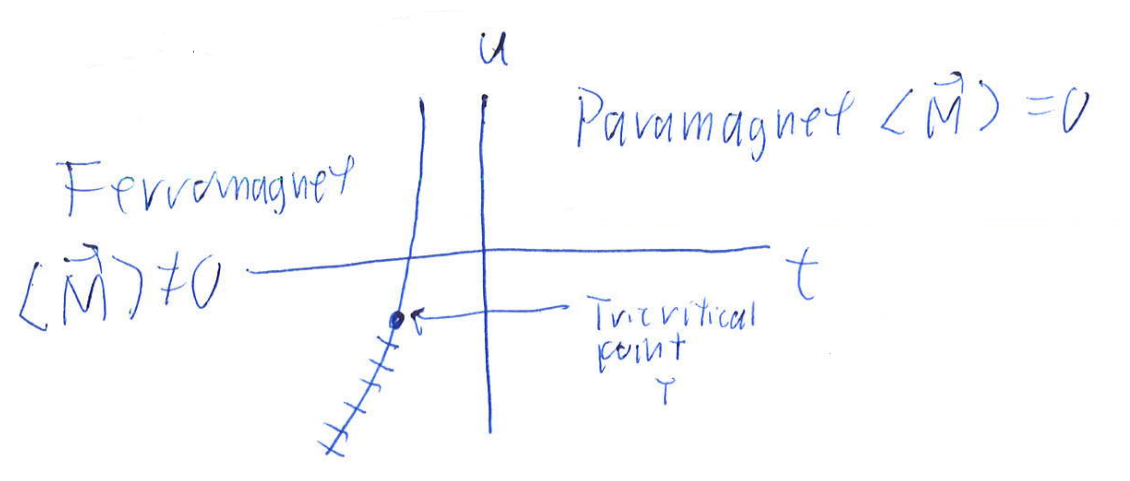
\includegraphics[scale=.75]{fig1}
    \centering
    \caption{$u-t$ Phase Diagram}
    \label{fig1}
\end{figure}
\begin{enumerate}[label=(\alph*)]
    \item Show, using mean-field theory, that the phase diagram in the $u-t$ plane, \underline{including} $u<0$, has the topology shown in Figure \ref{fig1}, where the crossed line denotes a first order transition, and the uncrossed line denotes a second order transition.
        The tricritical point $T$ separates the two types of transition. Figure \ref{fig1}, while ``topologically'' correct, does \textit{not necessarily} have the phase boundaries, and the tricritical point, in the right places.
        Your job, in this part of the problem, is to figure out where mean field theory says they are.
    \item Now do RG on this problem for small $u$ and $w$, and figure out where the phase boundaries and tricritical point are.
        In particular, find the upper critical dimension $d_{\text{uc}}^T$ for the fixed point controlling the tricritical point itself.
    \item Calculate the size of the first order jump in $\abs{\vec{M}}$ near the tricritical point, and show that it obeys the scaling law
        \begin{equation}
            \abs{\vec{M}}_{T_{1^{st}\text{order}}} \propto (u - u_T)^\phi
            \label{1.2}
            \tag{1.2}
        \end{equation}
        Calculate the exponent $\phi$ for $d>d_{\text{uc}}^T$; $d = d_{\text{uc}}^T - \epsilon$ with $\epsilon \ll 1$ and $d=3$.
\end{enumerate}

\section*{Problem 4}
In a uniaxial crystal, the Landau Hamiltonian for the magnetization can lack symmetry between one of the components (call it $z$) and all of the others, leading to a Landau Hamiltonian of the so-called ``spin-flop'' form:
\begin{equation}
    H = \int \dd^4 r \left[ \frac{t}{2}\abs{\vec{M}}^2 + u\abs{\vec{M}}^4 + \frac{l}{2}\abs{\vec{\nabla}\vec{M}}^2 + gM_z^2 \right].
    \label{2.1}
    \tag{2.1}
\end{equation}
Here $\vec{M}$ has $n>2$ components.
\begin{enumerate}[label=(\alph*)]
    \item Find the ``mean-field'' phase diagram for this model in the $(t,g)$ plane. Identify all of the phases; in particular, if $\ev{\vec{M}} \neq 0$ in any of them, say which way it points.
    \item Derive the RG recursion relations for this model in $d=4-\epsilon$.
    \item Using the results of (b), find the phase diagram in $d=4-\epsilon$ dimensions. In particular, identify the universality classes of any \nth{2} order transitions, and show that there is a point in the phase diagram where two second order transitions meet at a first order boundary, like so:
    \begin{figure}[H]
        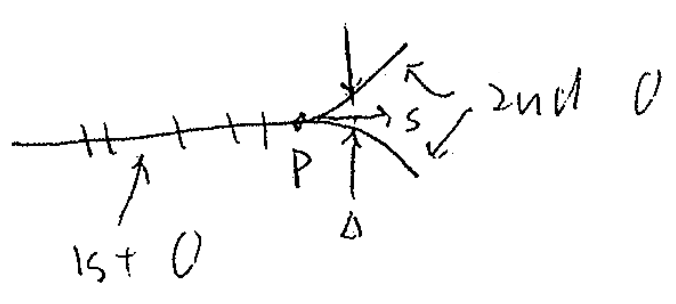
\includegraphics[scale=1]{fig2}
        \centering
        \caption{Two \nth{2} transitions meeting at a \nth{1} order boundary}
        \label{fig2}
    \end{figure}
    Show that the width $\Delta$ of the sliver of the phase between the two \nth{2} order boundaries grows as a function of distance $s$ away from the point $P$ where the three phase boundaries meet like $\Delta \propto s^\phi$, and calculate the ``crossover exponent'' $\phi$ to \nth{1} order in $\epsilon$. \\
    (i.e. $\phi = a + b\epsilon + O(\epsilon^2)$, you must calculate $a$ and $b$.)
\end{enumerate}


\end{document}